\section{Einbetten und Dualisieren}

\textbf{Einbettung} = Äquivalenzklasse von planaren Zeichnungen
\begin{center}
	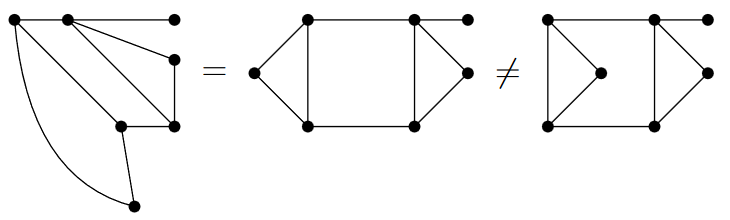
\includegraphics[width=0.4\textwidth]{images/einbettung.png}
\end{center}

\textbf{Definition}: Sei $G = (V, E)$ ein zusammenhängender Graph mit einer planaren Zeichnung.
Die \textbf{(kombinatorische) Einbettung} ist 
\begin{itemize}
	\item für jeden Knoten $v$ die zyklische (cw = \enquote{clockwise}) Reihenfolge der inzidenten Halbkanten an $v$
	\item für jede Facette $f$ die zykl. (cw) Reihenfolge der inzidenten Kantenseiten an $f$
\end{itemize}

Betrachte dafür beliebige Orientierung der Kanten und man erhält Halbkanten $e^{\text{in}}$ und $e^{\text{out}}$ sowie Kantenseiten $e^{\text{left}}$ und $e^{\text{right}}$ von $e$
\begin{center}
	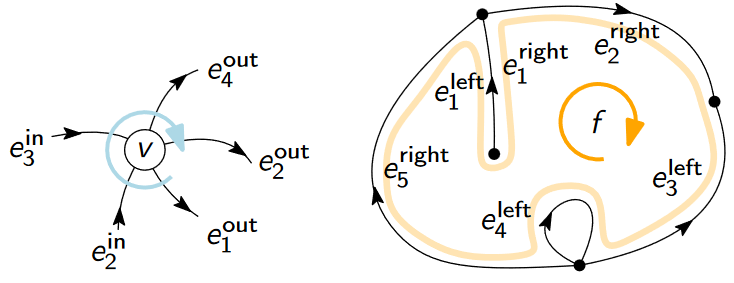
\includegraphics[width=0.5\textwidth]{images/einbettung-2.png}
\end{center}
\bigskip
Alle Zeichnungen mit der gleichen Einbettung sind äquivalent.\\

\textbf{Definition}: Sei $G = (V, E)$ ein zusammenhängender Graph mit einer festen Einbettung und Facettenmenge $F$. 
Der \textbf{Dualgraph} $G^* = (V^*, E^*)$ ist
\begin{itemize}
	\item $V^* = F$, das heißt, $f \in F \mapsto v_f \in V^*$
	\item für jede Kante $e \in E$ läuft die duale Kante $e^*$ zwischen der Facette an $e^{\text{left}}$ und der an $e^{\text{right}}$
\end{itemize}
\begin{center}
	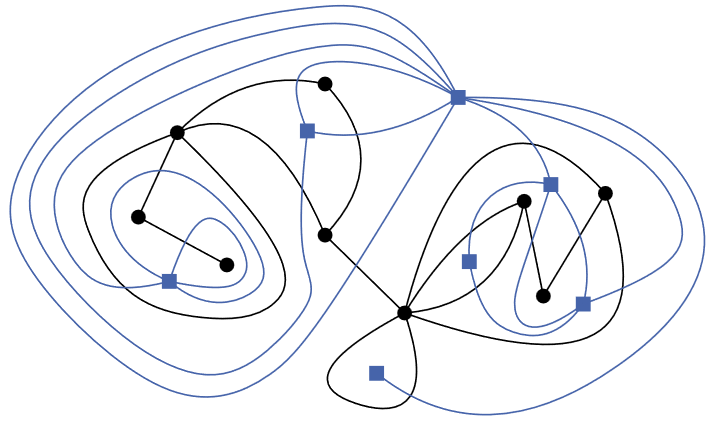
\includegraphics[width=0.4\textwidth]{images/dualgraph.png}
\end{center}

Die Einbettung des \textbf{Primalgraphen} $G = (V, E)$ induziert eine Einbettung des \textbf{Dualgraphen} $G^* = (V^*, E^*)$:
\begin{center}
	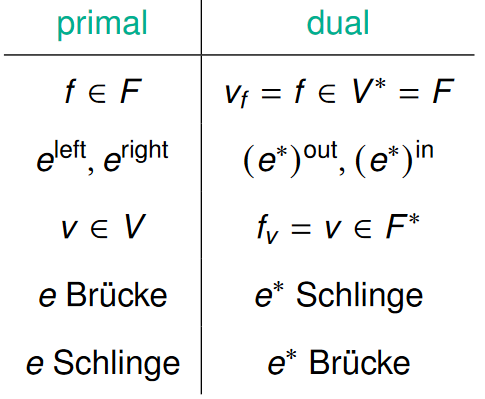
\includegraphics[width=0.3\textwidth]{images/primal-dual.png}
\end{center}
\bigskip
\textbf{Bemerkungen}: 
\begin{itemize}
	\item Der Dualgraph $G^*$ ist immer zusammenhängend
	\item Falls $G$ zusammenhängend ist, gilt $G = (G^*)^*$
	\item Für jede Einbettung von $G$ und jede Facette $f$ gibt es eine planare Zeichnung mit dieser Einbettung und $f$ als äußere Facette
\end{itemize}